\chapter*{Method - Redo}

In this chapter the method used to conduct this Master thesis will be described. The entire method is broken down into several different processes and sub processes to better structure and describe, this is illustrated in \ref{fig:Method_process}. Each individual process has an outcome which is needed as input in the next process. 

\begin{figure}[H]
    \centering
    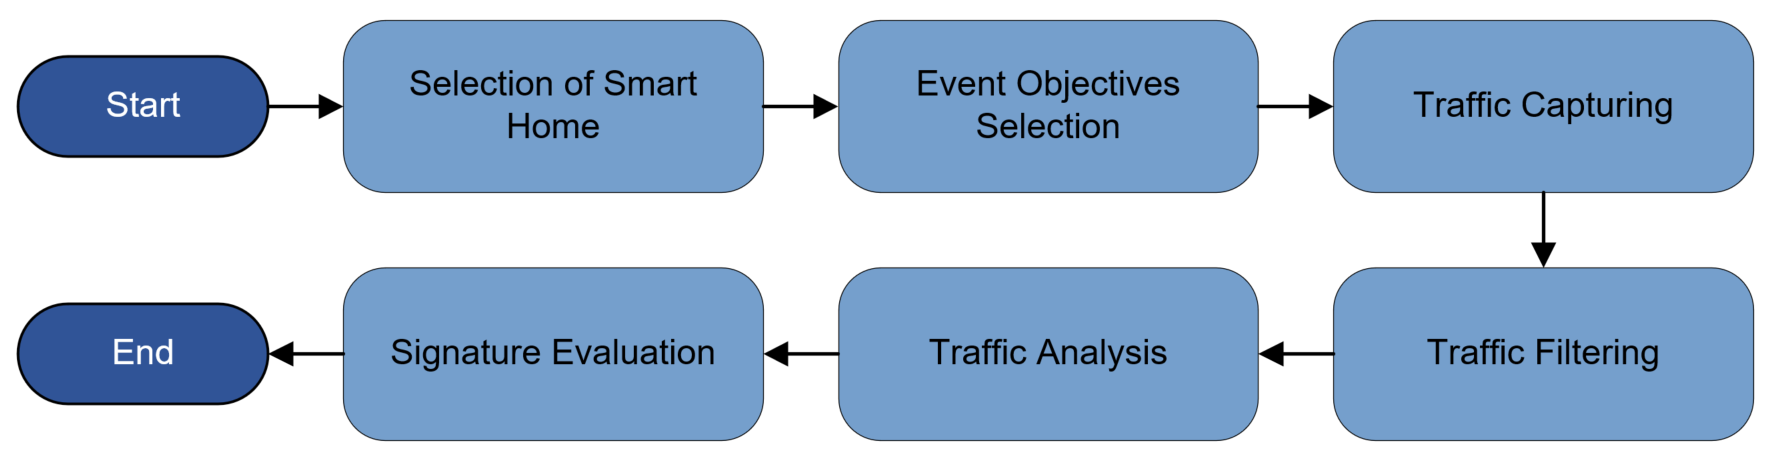
\includegraphics[width=\textwidth]{figures/Method_process.png}
    \caption{Overall phases }
    \label{fig:Method_process}
\end{figure}


\section{Device and Environment Selection}
With limited resources it is important to find the best satiable deceives for the thesis project. Since all the testing and analysis is based on the data generated by the robot vacuum cleaner, it will be selected first. To ensure that the thesis is relevant there is some requirements that is created.

\begin{figure}[H]
    \centering
    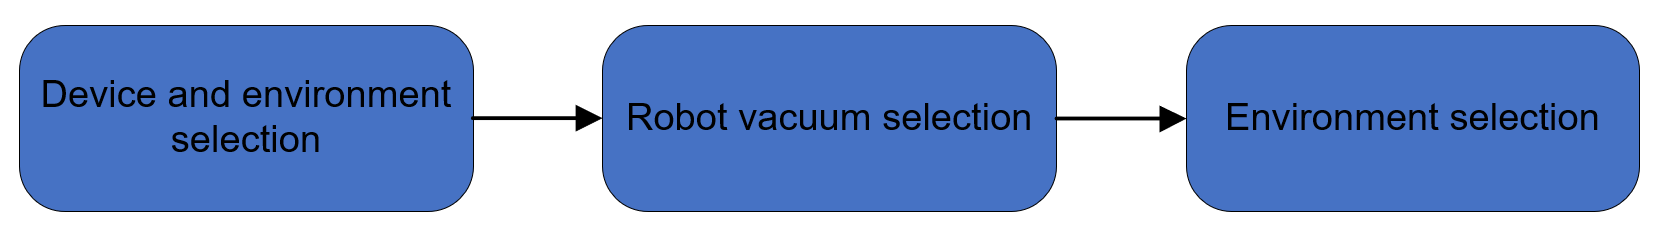
\includegraphics[width=\textwidth]{figures/DeviceSelectionProcess.png}
    \caption{Device Selection Process}
    \label{fig:DeviceSelectionProcess}
\end{figure}

\subsection{Selection Robot vacuum cleaner}
\begin{itemize}
    \item \textbf{Communication protocol:} Wi-Fi is the most wide spread communication protocol in today's IT infrastructure, as well as in Smart home \cite{robotsel1}. Eavesdropping devices and analysis tools are also more available for IEEE.802.11 and network layers higher in the OSI model \cite{osimodel}.
    
    \item \textbf{Smart Home Features:} The robot vacuum cleaner need to have several different smart home features. As more features available the more attribution and potential information can be extracted.This includes as application, which is more likely to produce traffic towards an external services, potentially exposing data \cite{robotsel4}.
    
    \item \textbf{Popularity:} The prevalence of different vendors and models will vary, and the popularity of the selected vacuum cleaner will impact the relevance of this research, the more devices used, the more smart home will be effected of the research's result. 
\end{itemize}

Data and ratings from these three robot vacuum cleaner review sites was used \cite{robotsel11}\cite{robotsel12}\cite{robotsel13}. The summary of all these reviews will be used to determine most reliable vacuum cleaner vendors. To determine the popularity of the different brands, statistics about number of downloads and ratings is gathered from Google Play \cite{GooglePlay} and compared.
Models within the assortment of the two highest scoring vendors will be compared and selected, based on the overall criteria and with the use of \cite{robotsel9}

\subsection{Result selection robot vacuum cleaner}

Results from thhe review sites shows that the two best robot vaccum cleaner vendors is Irobot and Roborock \ref{tab:RobotVacuumselcetionReviewSites}. 

\begin{table}[H]
    \centering
    \begin{subtable}[b]{0.45\linewidth}
        \centering
        \caption{Results from review-site \cite{robotsel11}}
        \label{tab:RobotReviw1}
        \begin{tabular}{|l|l|}
            \hline 
            \textbf{Vendor} & \textbf{Number on top ten} \\ \hline
            Irobot      & 3                 \\                   \hline
            Roborock    & 3                 \\                   \hline
            Neatsvor    & 0                 \\                   \hline
            Ecovacs     & 0                 \\                   \hline
            iLife       & 2                 \\                   \hline
        \end{tabular}
    \end{subtable}
    \hspace{0.5cm}
    \begin{subtable}[b]{0.45\linewidth}
        \centering
        \caption{Results from review-site \cite{robotsel12}}
        \label{tab:RobotReviw2}
        \begin{tabular}{|l|l|}
            \hline
            \textbf{Vendor}    & \textbf{Number on top ten} \\ \hline
            Irobot      & 2                 \\                   \hline
            Roborock    & 2                 \\                   \hline
            Neatsvor    & 0                 \\                   \hline
            Ecovacs     & 2                 \\                   \hline
            iLife       & 1                 \\                   \hline
        \end{tabular}
    \end{subtable}
    \begin{subtable}[b]{0.45\linewidth}
        \centering
        \caption{Results from review-site \cite{robotsel13}}
        \label{tab:RobotReviw2}
        \begin{tabular}{|l|l|}
            \hline
            \textbf{Vendor}    & \textbf{Number on top ten} \\ \hline
            Irobot      & 2                 \\                   \hline
            Roborock    & 2                 \\                   \hline
            Neatsvor    & 3                 \\                   \hline
            Ecovacs     & 1                 \\                   \hline
            iLife       & 0                 \\                   \hline
        \end{tabular}
    \end{subtable}
    \hspace{0.5cm}
    \begin{subtable}[b]{0.45\linewidth}
        \centering
        \caption{Summary of all review-sites}
        \label{tab:RobotReviw2}
        \begin{tabular}{|l|l|}
            \hline
            \textbf{Vendor}    & \textbf{Number on top ten} \\ \hline
            Irobot      & 7                 \\                   \hline
            Roborock    & 7                 \\                   \hline
            Neatsvor    & 3                 \\                   \hline
            Ecovacs     & 3                 \\                   \hline
            iLife       & 3                 \\                   \hline
        \end{tabular}
    \end{subtable}
    \label{tab:RobotVacuumselcetionReviewSites}
    \caption{Robot vacuum selection review-site}
\end{table}

Application related different vendors' robot vacuum cleaner is presented in \ref{tab:VendorApplicationStat}. It is worth mentioning that the "Smart Life" application used to control the Neatsvor is used to integrate the entire smart home and not just a robot vacuum cleaner. 

\begin{table}[H]
\centering
\caption{Vendor application statistics}
\label{tab:VendorApplicationStat}
\begin{tabular}{|c|c|c|c|}
\hline
\textbf{Vendor} & \textbf{Application} & \textbf{Downloads} & \textbf{Rating} \\ \hline
Irobot          & Irobot Home          & 5 million +        & 4,0/5,0         \\ \hline
Roborock        & Roborock             & 1 million +        & 4,6/5,0         \\ \hline
Neatsvor        & Smart Life           & 10 million +       & 4,5/5,0         \\ \hline
Ecovacs         & Ecovacs Home         & 1 million +        & 2,5/5,0         \\ \hline
iLife           & iLifehome            & 50 thousand +      & NA              \\ \hline
\end{tabular}
\end{table}
Both Irobot and Roborock received seven recommendations, which was significantly higher than the other three vendors on the list, each of which had only three representations. Additionally, both vendors were referenced in all three review sites, which strengthens their credibility. 

In the application download and ratings analysis, the Neatsvor application had over 10 million downloads. However, this application is more focused on smart home integration, and the high number of downloads is likely not solely due to the robot vacuum cleaner. Meanwhile, Evacos home received a 2.5/5.0 rating, and despite having a similar number of downloads as Roborock, it fell short in the selection process. Hence, Irobot and Roborock emerged as the two most relevant vendors. In a comparison of their products, it was found that the Irobot Roomba i7 and Roborock S6 were the best suitable robots according to our requirements \cite{robotsel8} \cite{robotsel6}. The comparison was conducted using the website \cite{robotsel9}, which is presented in Table \ref{tab:IrobotRoborockComparison}.

\begin{table}[H]
\centering
\caption{Irobot and Roborock comaprison}
\label{tab:IrobotRoborockComparison}
\begin{tabular}{|p{0.45\textwidth}|p{0.45\textwidth}|}
\hline
\multicolumn{1}{|c|}{\textbf{Irobot roomba i7}}        & \multicolumn{1}{c|}{\textbf{Roborock s6}}                \\ \hline
Camera   and odometry for navigation                   & Map   discovery, and storage of floorplan                \\ \hline
Cleaning   suggestions by the application              & Scheduling                                               \\ \hline
Zone   based cleaning                                  & No   map zones, mapping zones                            \\ \hline
Seasonal   cleaning                                    & Real-time   tracking                                     \\ \hline
Pet   detection                                        & LDS   sensor for mapping and navigation                  \\ \hline
SRR   rating App features 71, Usability and control 69 & SRR   rating: App features 100, Control and usability 71 \\ \hline
Price:   3990kr                                        & Price:   3990kr                                          \\ \hline
\end{tabular}
\end{table}

Irobot roomba i7 and Roborck S6 have similar reviews and rating all over, and they both have a sufficient number of smart home features required in this thesis. The fact that the Irobot application is downloaded 5 times more than the Roborock was the decisive factor, and Irobot roomba i7 will be used during this research. 

\subsection{Environment selection}
The rest of the research environment have to support and allow traffic eavesdropping and analysis, of the Irobot Roomba i7.  Important factors to support in research environment:

\begin{itemize}
    \item \textbf{IEEE.802.11 WI-FI network}
    \item \textbf{Internet connection}
    \item \textbf{Different physical rooms}
\end{itemize}

\subsubsection{Physical environment}
To ensure the validity of the results across diverse settings, the testing will be conducted in two different home environments situated in separate cities. The Robot vacuum cleaner will be configured from factory defaults for each research environment. Both home environments have independent Internet access, provided by distinct external Internet Service Providers (ISPs). To control the duration of each test, the trials will be restricted to the room with the ISP router. As the floor space in this room is smaller, the cleaning process will be relatively shorter. An illustration of the two distinct smart home environments is provided below in \ref{fig:SmartHomeEnvironments}.

\begin{figure}[H]
    \centering
    \begin{subfigure}[b]{0.80\textwidth}
        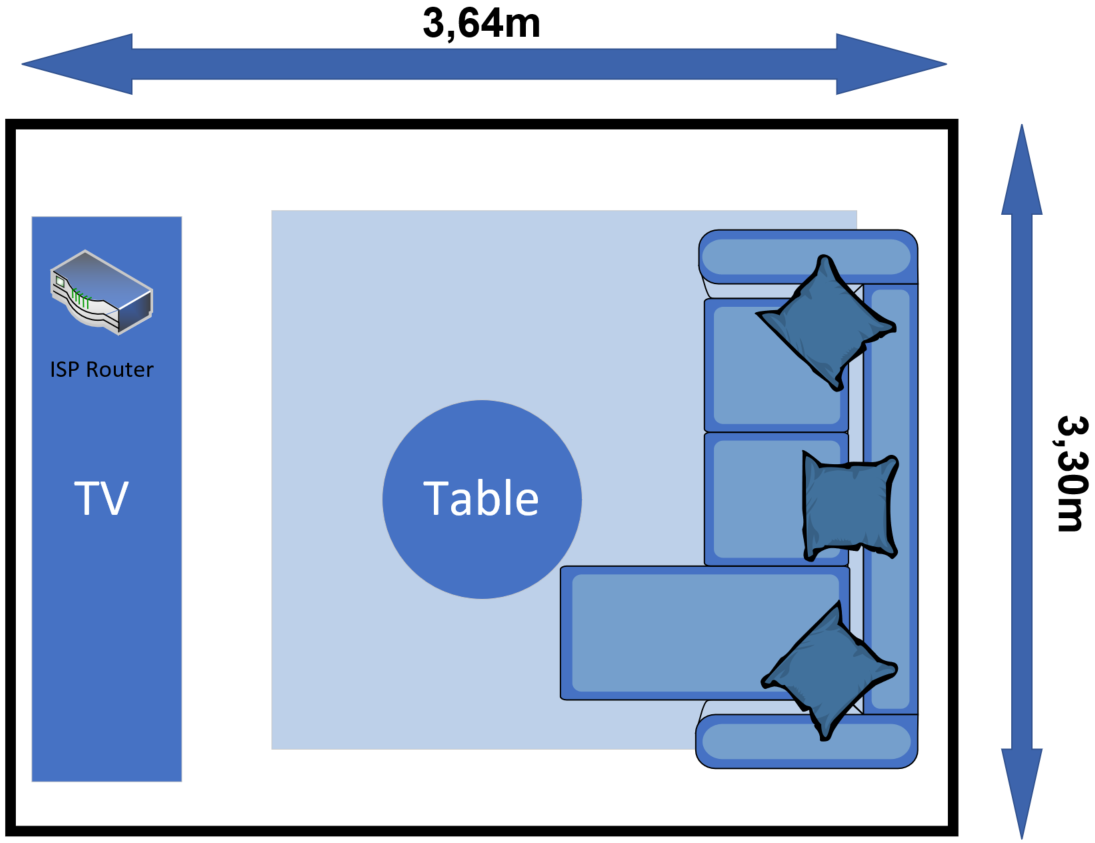
\includegraphics[width=\textwidth]{figures/Environment1.png}
        \caption{Research environment 1}
        \label{fig:Environment1}
    \end{subfigure}
    \hfill
    \begin{subfigure}[b]{0.80\textwidth}
        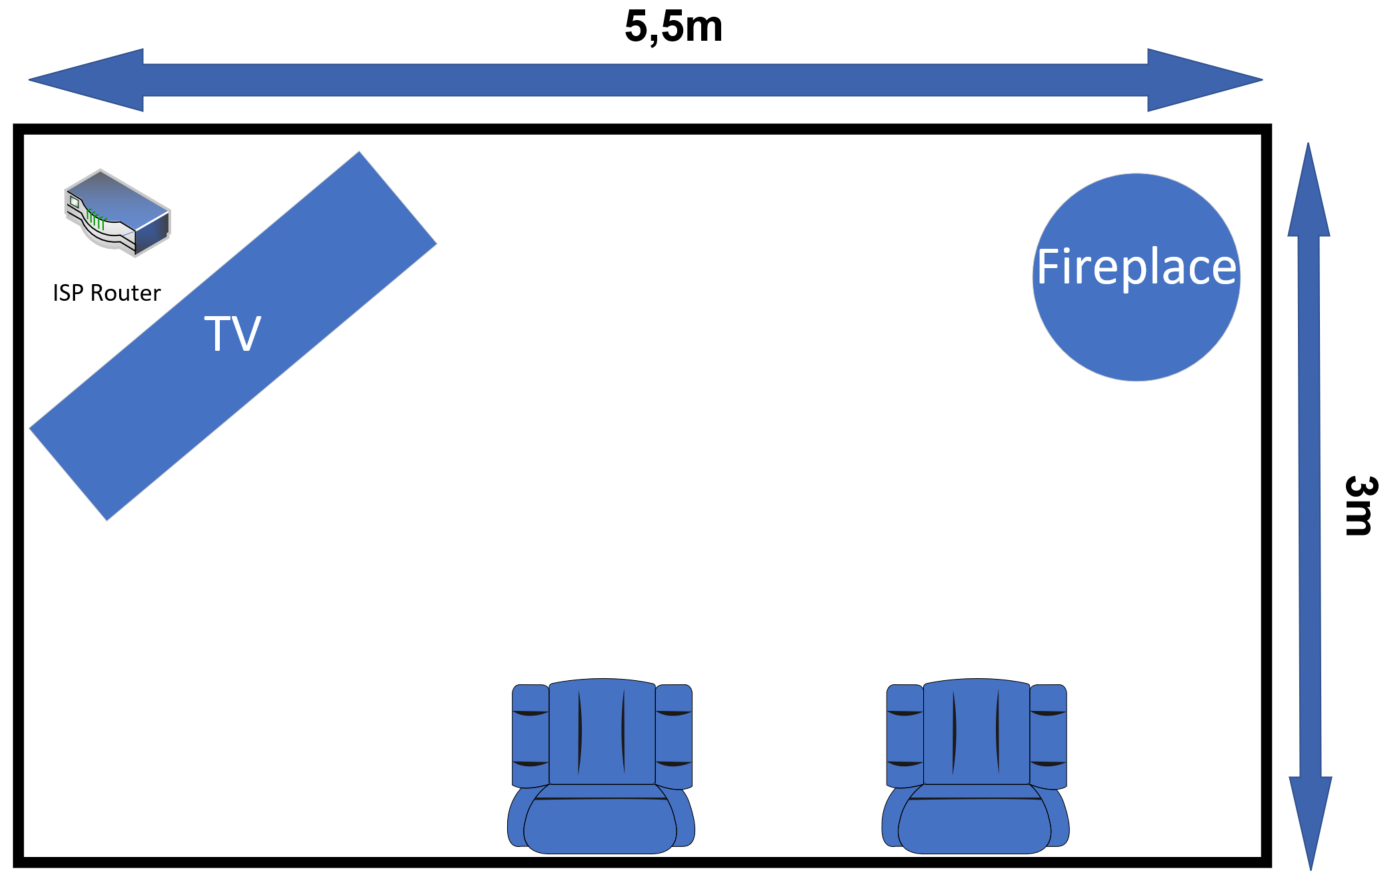
\includegraphics[width=\textwidth]{figures/Environment2.png}
        \caption{Environment 2}
        \label{fig:Environmet2}
    \end{subfigure}
    \caption{Smart Home environments }
    \label{fig:SmartHomeEnvironments}
\end{figure}

\subsubsection{Capturing and Analysis platform}
For the capturing and analysis platfrom there is some requirements that needs to be fulfilled. Due to limited resources the platforms need to be available for limited cost. 

\begin{itemize}
    \item \textbf{Capturing platform} needs to be able to operate autonomously, due to continuously capturing of events. It needs software that enables capturing of wireless IEEE.802.11 and wired traffic IEEE.802.3 at the same time. This data will need to be transferred from the device to the analysis platform.
    \item \textbf{Analysis platform} needs to have tools analysis the traffic, based on the format of the capturing tool. 
\end{itemize}

As capturing platform the Raspberry PI 3b+ is chosen, this was available form free through the authors' employer. This device is created to run autonomous, as OS the Kali Linux is installed. This is a open source operating system, including several different tools to capture and analyse traffic and has has an OS-version designed for Raspberry PI \cite{kalidownload}. To enable capturing of wireless traffic the wireless network interface card needs to be in \textit{Monitor mode}. For Kali Linux the \textit{LINK TL-WN722N V2/V3} is recommended by \cite{Kali_monitormode_guide}, and is therefore used in this research. 
Analysis platform is a HP Elitebook due to availability. Is runs Windows 11 OS which is compatible with several different tools for capturing and analysis.

\subsubsection{Environment infrastructure}
This research will include eavesdropping of wireless traffic and wired WAN traffic. The two different smart home environments only includes a single ISP router providing both Internet connection and Wi-Fi, and does not have a features allowing the captuing platfrom to eavsdropp the wired traffic generated by the robot vacuum cleaner. Additional infrastructure is therefore added: 
\begin{itemize}
    \item \textbf{Wireless access point:} This access point will create a new SSID only to be used by the Robot vacuum cleaner, this isolates the vacuum cleaner from potential impact from other devices on the WLAN/LAN. The access point will also use Network address translation and translate all traffic to one singe IP address. With this setup, all traffic with the source address of the access point will be either the access point itself, or the robot vacuum cleaner.
    \item \textbf{LAN switch:} The LAN switch will be directly connected to both the access point and the ISP router. All Internet traffic will therefore be transmitted though the switch. A SPAN port is configured on the switch, this port will monitor all traffic on the port connected to the access point, and duplicate this flow to the port connected to the capturing platform. This setup is illustrated in \ref{fig:WLAN_LAN_setup}
\end{itemize}

\begin{figure}[H]
    \centering
    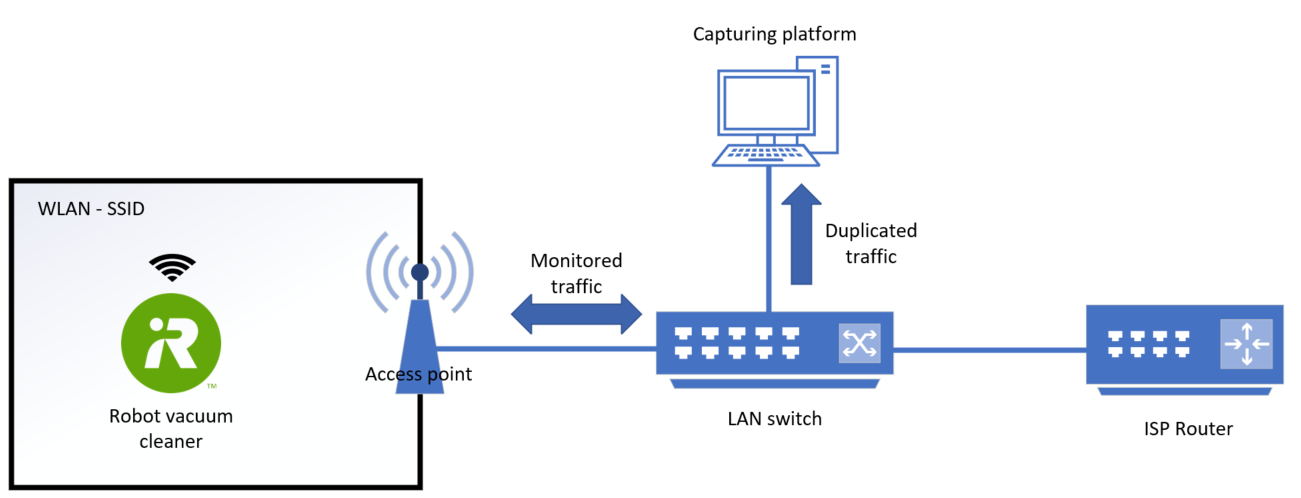
\includegraphics[width=\textwidth]{figures/WLAN_LAN_setup.png}
    \caption{Smart Home infrastructure}
    \label{fig:WLAN_LAN_setup}
\end{figure}



\subsubsection{Capturing and Analysis tools}
Capturing and analysis tools need to be compatible with each other. Stored format from the capturing process needs to be readable in the analysis phase. Tools for these kinds of tasks are many. Whireshark is a widely used network protocol analyser, it allows network capturing and analysis in real-time. It can be used for deep header inspection in all network layers which is not encrypted before the capturing, this makes it a valuable tool for network and security purposes. The application can perform basic identification of a wide range of different protocols across networks layers as well as statistics about the traffic flow. This software is also default installed on Kali Linux OS. Wireshark is also available for Windows on \cite{wireshark_download_2016}.
Tshark is a sub-software included in wireshark and the process which is used to capture traffic on the dedicated network interfaces. This software can be used to capture traffic through CLI. In this process it is possible to define capturing filters which only store traffic that is interesting for the analysis phase.


\section{Traffic capturing}
This section will describe the tools used for traffic capturing, tests and the process of how the capturing process is executed. All capturing will be executed on the capturing platform, both LAN and WLAN traffic is captured simultaneously. This enables correlation of the traffic for the same event.  

\begin{figure}[H]
    \centering
    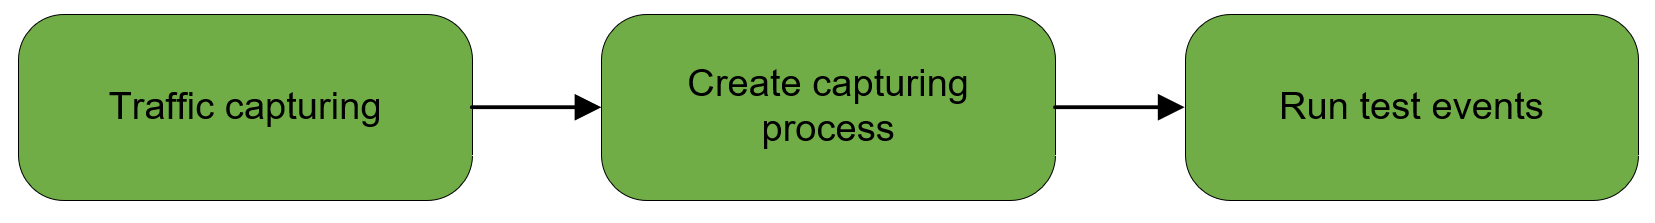
\includegraphics[width=\textwidth]{figures/TrafficCapturingProcess.png}
    \caption{Traffic Capturing Process}
    \label{fig:TrafficCapturingProcess}
\end{figure}

\subsection{Captuing tools}
Tshark will be used as the capturing tools for both wireless and wired traffic. Two Tshark instances will run simultaneously on the capturing platform. The Tshark filter syntax used for both capturing streams is: 
\\
tshark [ -i <capture interface>|- ] [ -f <capture filter> ] [ -w <outfile>|- ]
\\
The captuing platform has three different NICs:
\begin{itemize}
    \item \textbf{eth0,} is the wired IEEE 802.3 interface which is connected to the SPAN port of the LAN switch.
    \item \textbf{wlan0,} is the buildt in IEEE 802.11 interface on the Raspberry PI.
    \item  \textbf{wlan1,} external IEE 802.11 adapter which is configured to monitor mode.
\end{itemize}

LAN Tshark command:
\\
sudo tshark -i wlan1 -f 'ip.host "WAN address' -w output.pcap
\\
WLAN Tshark command:
\\
sudo tshark -i wlan1 -f 'eth.host "MAC address' -w output.pcap
\\

\subsection{Capturing process}
The capturing process will be similar for all events, this will create a better foundation to compare the different test results. \ref{fig:captuingprocess} illustrate the entire process.
\begin{enumerate}
    \item Star both LAN and WLAN capture, in separate Tshark processes.
    \item Trigger events according to test event matrix. Note event Start and End during the testing. 
    \item If pcap file exceeds 500MB, stop capture, and start new LAN and WLAN capture.
    \item When testing in environment is finished, stop capture. 
    \item Transfer files to analysis platform
\end{enumerate}
   

\begin{figure}[H]
    \centering
    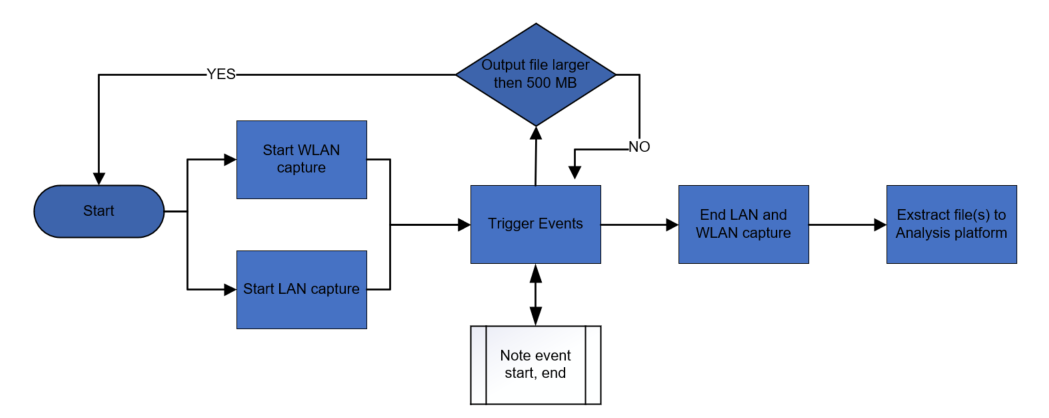
\includegraphics[width=\textwidth]{figures/Event triggering process.png}
    \caption{Capturing process}
    \label{fig:captuingprocess}
\end{figure}

\subsection{Events tests}
This section will describe the different features that is included in the research and the overall event triggering process. Each test will be executed at least n times for each of the two environments. N is the number of event which is decided to be sufficient to extract signatures with human manual analysis. The overall event triggering process is illustrated in \ref{fig:EventTriggeringProcess}

\begin{figure}[H]
    \centering
    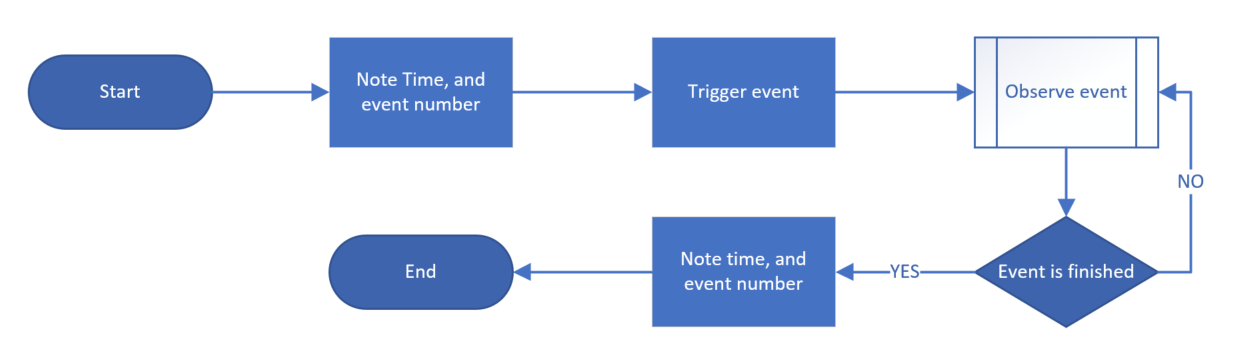
\includegraphics[width=\textwidth]{figures/EventTriggeringProcess.png}
    \caption{Capturing process}
    \label{fig:EventTriggeringProcess}
\end{figure}

\subsection{Event tests}
In this section all the different test flows will be described. This will make the tests and results more reproducible. 

\subsubsection{Standby Traffic}
This test is executed to identify network traffic generated to the robot vacuum cleaner in a standby mode. This means that there is no interaction done by human. 

\begin{itemize}
    \item \textbf{Event flow} \begin{enumerate}
                                    \item Start captuing of LAN and WLAN traffic
                                    \item Wait 14 days without any human interaction
                                    \item Stop capturing
                                \end{enumerate}
    \item \textbf{Number of events:} 1
\end{itemize}

\subsubsection{Scheduled Cleaning}
Scheduled cleaning can be configured through the application. Users can schedule a cleaning, specifying area in the smart home, time which the cleaning should start, as well as how often this should occur. 
\begin{itemize}
    \item \textbf{Event flow} \begin{enumerate}
                                    \item Schedule cleaning outside of event capture
                                    \item Note the time when cleaning started
                                    \item Note when "finished cleaning" notification is received
                                \end{enumerate}
    \item \textbf{Number of events in each environment:} 10
\end{itemize}

\subsubsection{Automated cleaning}
Irobot has features to integrate other services as triggers for events. This includes IFFF location tracker, Agust smart lock system, ecobee termotat system, My Leviton smart home integration and MyQ garage system. In this research the IFFF location system will be used. Cleaning is then triggered when the users phone is x meters away from home, where x is between 100m and 1 km. 

\begin{itemize}
    \item \textbf{Event flow} \begin{enumerate}
                                    \item Configure automated cleaning outside of event capture
                                    \item Leave the smart home environment
                                    \item Note when cleaning notification is received
                                    \item Note when "finished cleaning" notification is received
                                \end{enumerate}
    \item \textbf{Number of events in each environment:} 10
\end{itemize}

\subsubsection{Application triggered cleaning}
In the application users can trigger cleaning. There is a predefined "clean all" option, if the user have not customized. Cleaning is triggered when the user is pressing a cleaning option in the application.

\begin{itemize}
    \item \textbf{Event flow} \begin{enumerate}
                                    \item Note time
                                    \item Open the application and trigger "clean all" event
                                    \item Note when "finished cleaning" notification is received
                                \end{enumerate}
    \item \textbf{Number of events in each environment:} 10
\end{itemize}

\subsubsection{Physical triggered cleaning}
The Irobot roomba i7 has a physical cleaning button on top of the vacuum cleaner. A "clean all" vent is triggered when this button is pressed.

\begin{itemize}
    \item \textbf{Event flow} \begin{enumerate}
                                    \item Note time
                                    \item Press the physical clean button on the vacuum cleaner
                                    \item Note when "finished cleaning" notification is received
                                \end{enumerate}
    \item \textbf{Number of events in each environment:} 10
\end{itemize}

\subsubsection{Open application}
When the application is opened information will be displayed, through the application the user can interact and change setting. 

\begin{itemize}
    \item \textbf{Event flow} \begin{enumerate}
                                    \item Note time
                                    \item Open the application on the smart phone
                                    \item wait for some time
                                    \item Close application
                                    \item Note time
                                \end{enumerate}
    \item \textbf{Number of events in each environment:} 10
\end{itemize}

\subsubsection{Remove bin}
The Irobot roomba i7 has it own bin where dust is collected during clean. This can be removed if it is to be empty. The user will then have to physically remove and insert again. 

\begin{itemize}
    \item \textbf{Event flow} \begin{enumerate}
                                    \item Note time
                                    \item Remove the bin
                                    \item wait ta least 40 seconds
                                    \item Insert the bin
                                    \item Note time
                                \end{enumerate}
    \item \textbf{Number of events in each environment:} 10
\end{itemize}

\section{Traffic processing}
To make the processing feasible for the human mind there will be conducted some pre processing and filtering of the data. The standby traffic capture will be used for the initial processing, all traffic in this capture is either generated by the Access point or the robot vacuum cleaner. This initial processing will be done in Wireshark. Reoccurring traffic in the Standby capture can be filter out since they are not directly connected to an event that is triggered. All the identified traffic flows not relevant to events will be added to Wireshark capture filter \cite{wireshark}, and excluded from the display.

\begin{figure}[H]
    \centering
    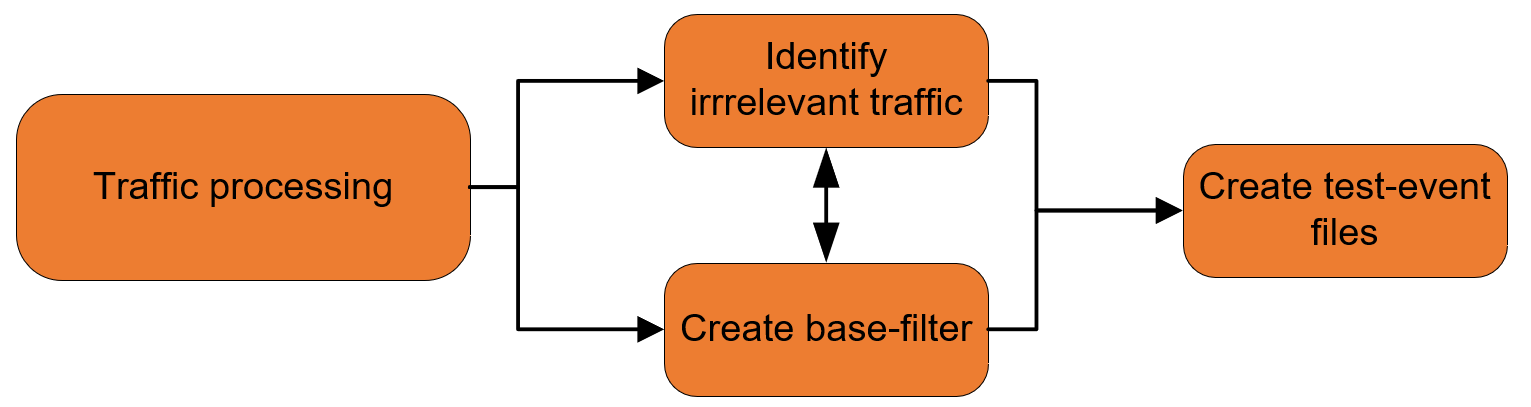
\includegraphics[width=\textwidth]{figures/TrafficProcessingProcess.png}
    \caption{Traffic processing Process}
    \label{fig:TrafficProcessingProcess}
\end{figure}


The Wireshark filter will be created with a series of if statements combined in a logical AND, or , not system. Each irrelevant traffic flow will be added to this combined filter. At the end of pre-processing a time filter will be added to create individual pcap files per event. This is to isolate the events in the analysis phase, this filter will use event start and end which was stored in the traffic capturing process. 

\textit{(frame.len >= " Month day, start-time") \&\& (frame.len <= "Month day, end-time")}

\begin{figure}[H]
    \centering
    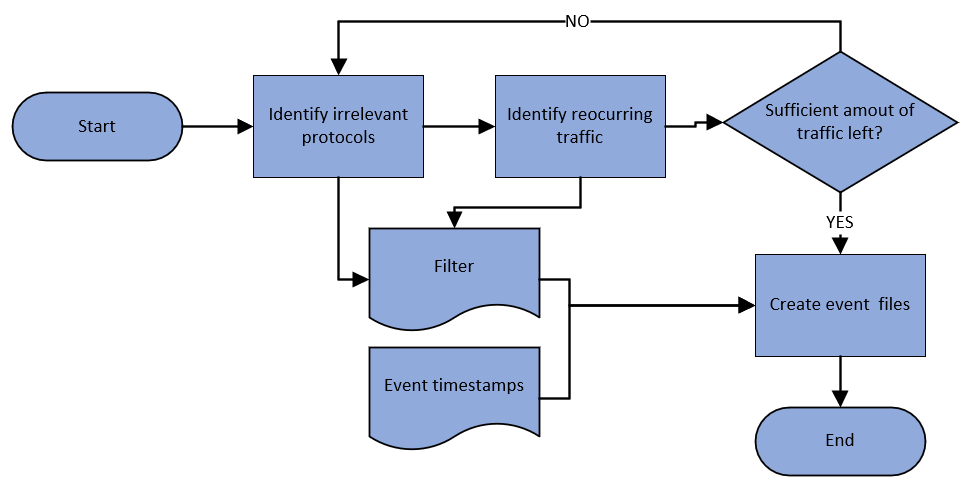
\includegraphics[width=\textwidth]{figures/TrafficprocessingFilter.png}
    \caption{Capturing process}
    \label{fig:<trafficProcessFilter}
\end{figure}

\section{Traffic Analysis}
The traffic analysis will be divided into three different processes, \textit{protocol and event relation, Traffic sequence identification and Overall event characteristics}. 

\begin{figure}[H]
    \centering
    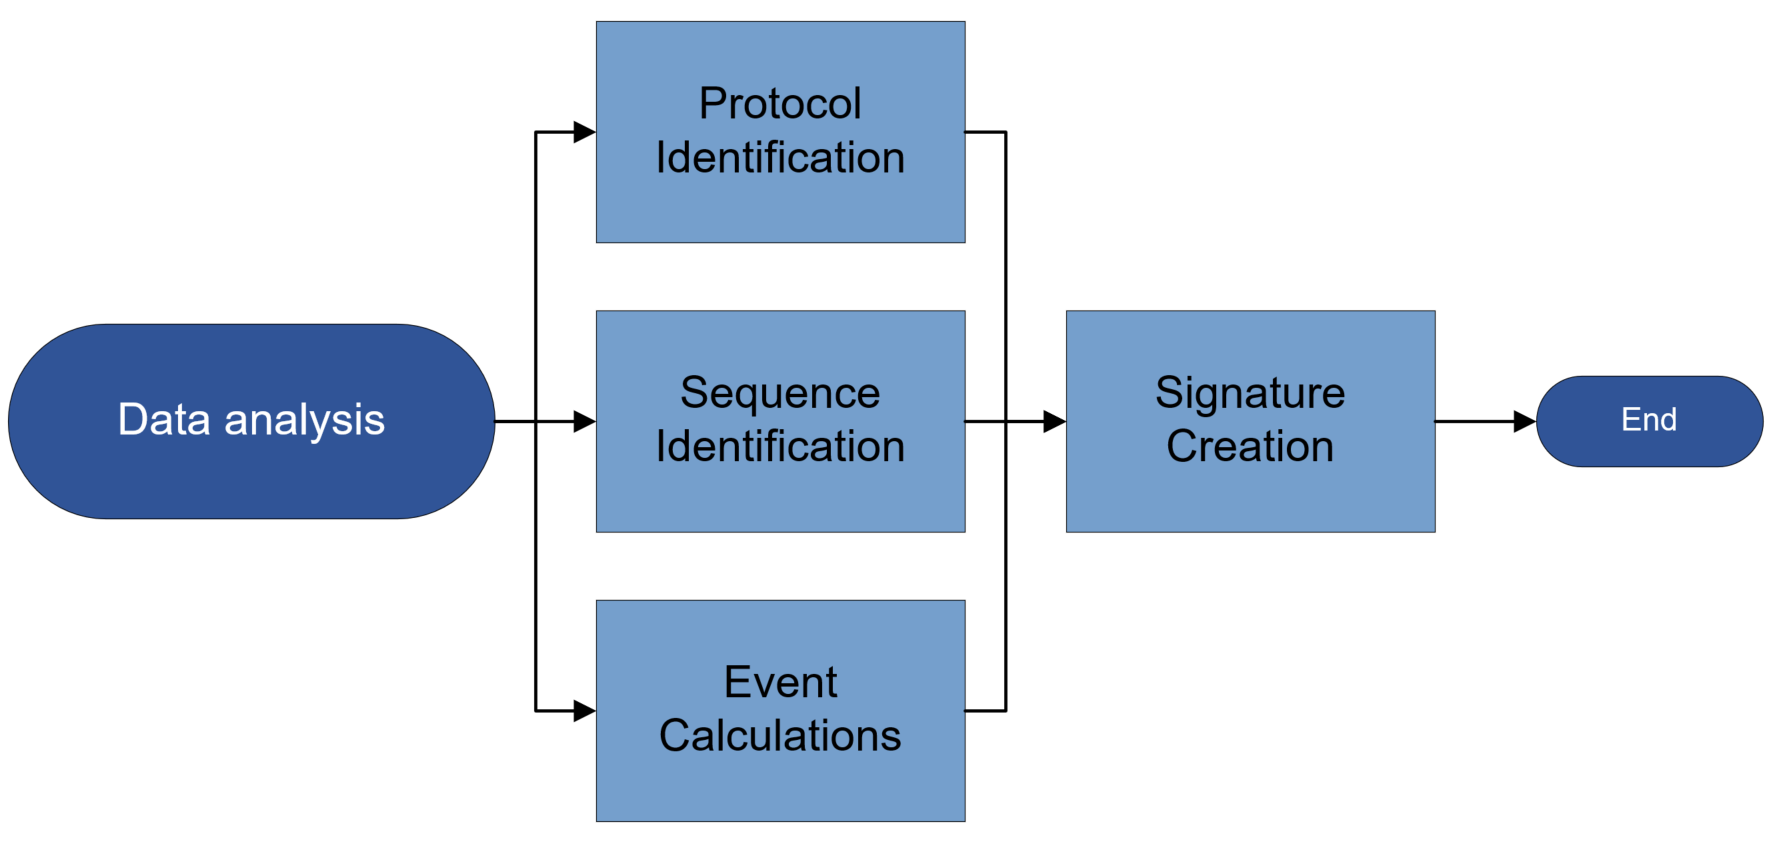
\includegraphics[width=\textwidth]{figures/TrafficAnalysisProcess.png}
    \caption{Traffic Analysis Process}
    \label{fig:TrafficAnalysisProcess}
\end{figure}

\subsection{Protocol event relation}
In this process Wireshark will be used to identify the different protocols in each event. Each identified protocol will then be looked at individually first, before combining findings in the overall event.

\subsection{Traffic sequence}
Other researches have used attributes in captured traffic flow to identify events. In this process the same approach as used in \cite{pingpong} will be done. Packet lengths around the time where the event was triggered. Three different types will be extracted: 
\begin{itemize}
    \item Packet lengths both directions.
    \item Packet lengths with Vacuum cleaner as source.
    \item Packet lengths with vacuum cleaner as destination.
\end{itemize}

\subsection{Overall event characteristics}
Each event has an overall characteristics, this data will be extracted and compared against the other event files. The data which will be compared is: 
\begin{itemize}
    \item Number of packets
    \item Total bytes
    \item Total bytes sent from vacuum cleaner
    \item Total bytes received as vacuum cleaner
    \item Different protocols
\end{itemize}

\subsection{Event signatures}
The output from the different identification processes will be compared and used to create suggestion for event signatures. These signatures will be created as conditions in a python script, and applied to the different event files to see if it is possible to identify the same signature in the event file. 
If the event is identified, the signature is testet on the other evetns' files to see if it will generate false positive. If the signature results in a success rate higher then x, it will be consider to be possible to identify. The logic will follow sudo code:
\\ 
\begin{lstlisting}
# Python code, Signeture detection
1. def Identify_event(event_file, event_confidence_variable):
2.     event_siganture = ['siganture']
3.     if event_signature is in eventfile:
4.         event_confident_variabel =+ x
5.     else
6.         None
7.     return evenr_confodence_variabel
\end{lstlisting}

\section{Signature detection and evaluation}
All signatures with higher success rate then x, will be included in the Human-learn:rule-based script. The detection algorithm has limitations, and can only identify one event per pcap file. For each event there will be a function checking for an event signature in the imported pcap file. It will follow this logic:
\\

\begin{lstlisting}
# Python code, Signeture detection
1. Main()
2.      #import event pcap file
3.      Capture = import(Event_file_x)
4.      #Run detection functions, and create confidence variables
5.      #eventX_confident_variable = eX_cv  
6.      e1_cv = identify_event1(Capture, event1_confodence_variable)
7.      e2_cv = identify_event2(Capture, event1_confodence_variable)
8.      e3_cv = identify_event3(Capture, event1_confodence_variable)
9.      e4_cv = identify_event4(Capture, event1_confodence_variable)
10.     e5_cv = identify_event5(Capture, event1_confodence_variable)
11.     e6_cv = identify_event6(Capture, event1_confodence_variable)
12.     #comapre event_confident_variables highest is event
13.     confident_variables = [list of all variables]
14.     for event in range(1,6)
15.          if confidentvariabels[event] is larger then last number
16.              largest = confidentvariabels[event]  
\end{lstlisting}

\subsection{Evaluation}
After completing the analysis and creating signature detection rules, a evaluation test will be done. The robot vacuum cleaner will be run in three new environment with, form factory defaults. Each event will be executed one time per new evaluation environment, within 30 minutes there will be executed an event. Our detection algorithm will then test is it is able to identify these events correctly. 